%This is a experiment example of ZhengXiaoyang's experiment report template

\documentclass[UTF8]{ctexart}
 
\usepackage{amsmath}
\usepackage{cases}
\usepackage{cite}
\usepackage{xeCJK}
\usepackage{graphicx}
\usepackage{siunitx}
\usepackage[margin=1in]{geometry}
\geometry{a4paper}
\usepackage{fancyhdr}
\pagestyle{fancy}
\fancyhf{}

\graphicspath{{picture/}}


\title{利用霍尔传感器测量磁场}
\graphicspath{{picture/}}


\title{利用霍尔传感器测量磁场}
\author{郑晓旸}
\date{\today}
\pagenumbering{arabic}

\begin{document}
%这里是文件的开头
\fancyhead[L]{郑晓旸}
\fancyhead[C]{磁场测量}
\fancyfoot[C]{\thepage}

\maketitle
\tableofcontents
\newpage

\section{实验目的}
    \begin{enumerate}
        \item 了解霍尔传感器的工作原理以及标定方法
        \item 研究亥姆霍兹线圈的磁场分布规律 
        \item 研究测量磁介质对磁场的分布的影响
    \end{enumerate}



\section{实验原理}

    \subsection{霍尔效应}
    
    霍尔效应是载流子在磁场中受到洛伦兹力而发生偏转,在材料两侧积累电荷从而形成霍尔电压的现象。如图\ref{fig:hall_effect}所示,设材料中载流子电荷量为 $q$,浓度为 $n$,在电流 $I_S$ 作用下沿 $x$ 方向运动,平均速度为 $v$。施加垂直磁场 $\vec{B}=(0,0,B)$ 后,载流子在洛伦兹力 $\vec{F}_L=q\vec{v}\times\vec{B}$ 作用下沿 $y$ 方向偏转,在两侧形成净电荷,产生横向电场 $\vec{E}=(0,E,0)$。当电场力 $\vec{F}_E=q\vec{E}$ 与洛伦兹力平衡时,载流子不再偏转,两侧电势差即为霍尔电压 $V_H$。
    
    \begin{figure}[htbp]
    \centering
    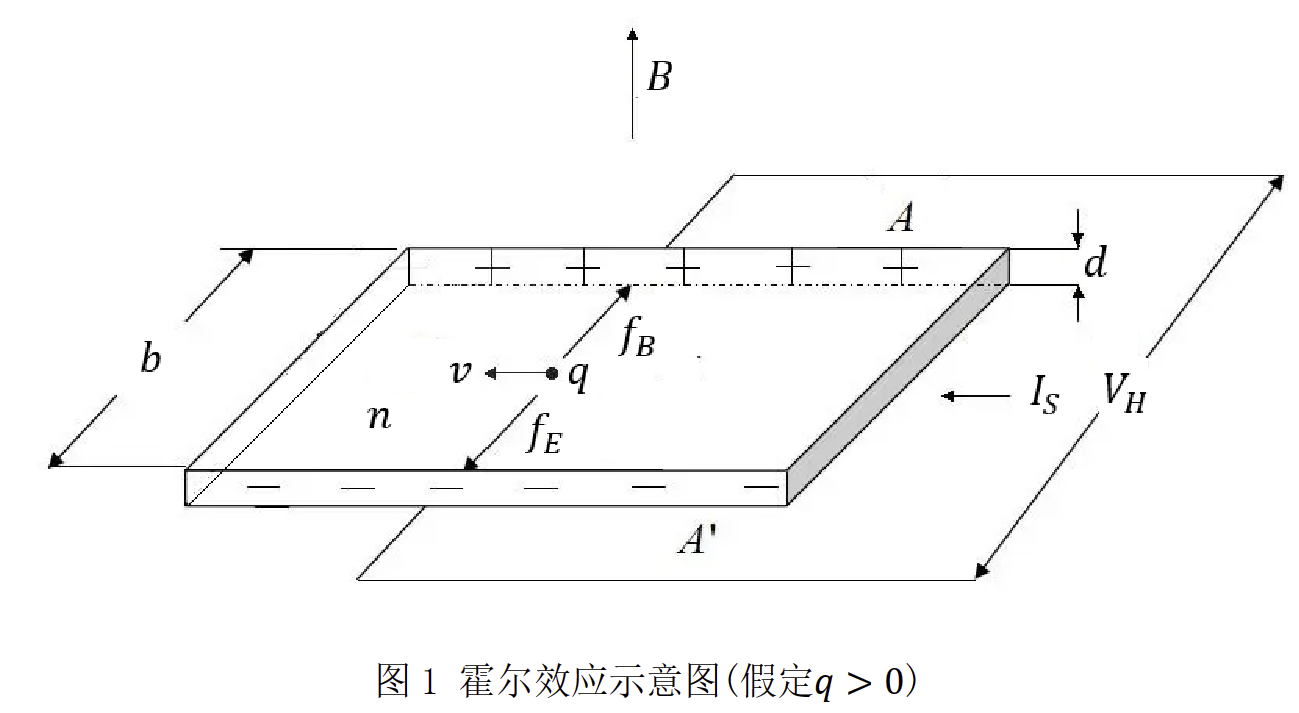
\includegraphics[width=0.7\textwidth]{hall_effect.png}
    \caption{霍尔效应示意图}
    \label{fig:hall_effect}
    \end{figure}
    
    由洛伦兹力和电场力平衡条件可得:
    
    \begin{equation}
    qvB = qE \Rightarrow E=vB
    \end{equation}
    
    而
    \begin{equation}
    V_H = Ed = vBd
    \end{equation}
    
    结合材料中电流密度 $j=qnv$,载流子速度 $v=\frac{I_S}{qnbd}$,代入上式可得:
    
    \begin{equation}
    V_H = \frac{I_SB}{qnd} \equiv K_HI_SB
    \end{equation}
    
    其中 $K_H=\frac{1}{qnd}$ 为霍尔元件的灵敏度,与材料特性有关。
    
    在实际测量中,由于制作工艺和材料非理想性,霍尔电压往往混有其他效应的贡献:
    \begin{itemize}
      \item 不等位电动势 $U_p$:电极焊接位置不同,存在与 $I_S$ 成正比的电势差
      \item 爱廷豪森效应 $U_E$:载流子速度分布不均,磁场下偏转程度不同,两侧产生温差,热电偶效应电动势正比于 $I_SB$ 
      \item 能斯特效应 $U_N$:磁场存在时,材料纵向温差会产生横向电势差,正比于 $I_S^2B$
      \item 里奇-勒杜克效应 $U_R$:磁场存在时,材料横向温差会产生纵向温差,热电偶效应电动势正比于 $I_S^2B$
    \end{itemize}
    
    霍尔元件输出电压为以上各项的叠加:
    
    \begin{equation}
    U = V_H + U_p + U_E + U_N + U_R
    \end{equation}
    
    通过改变 $I_S$ 和 $B$ 的方向,可以消除 $U_p$、$U_N$ 和 $U_R$ 的影响:
    
    \begin{equation}
    V_H + U_E = \frac{1}{4}(U_{++} - U_{+-} + U_{--} - U_{-+})  
    \end{equation}
    
    其中下标 $++$、$+-$、$--$、$-+$ 分别表示 $I_S$ 和 $B$ 同向、$I_S$ 反向 $B$ 同向、$I_S$ 和 $B$ 反向、$I_S$ 同向 $B$ 反向。在 $|V_H| \gg |U_E|$ 时,可近似得到 $V_H$。
    
    \subsection{亥姆霍兹线圈的磁场分布}
    
    亥姆霍兹线圈由两个半径为 $R$、匝数为 $N$ 的同轴环形线圈组成,两线圈平面间距为 $R$,绕组方向相同,如图\ref{fig:helmholtz_coil}所示。当通以电流 $I_M$ 时,在轴线上产生较为均匀的磁场。
    
    \begin{figure}[htbp]
    \centering
    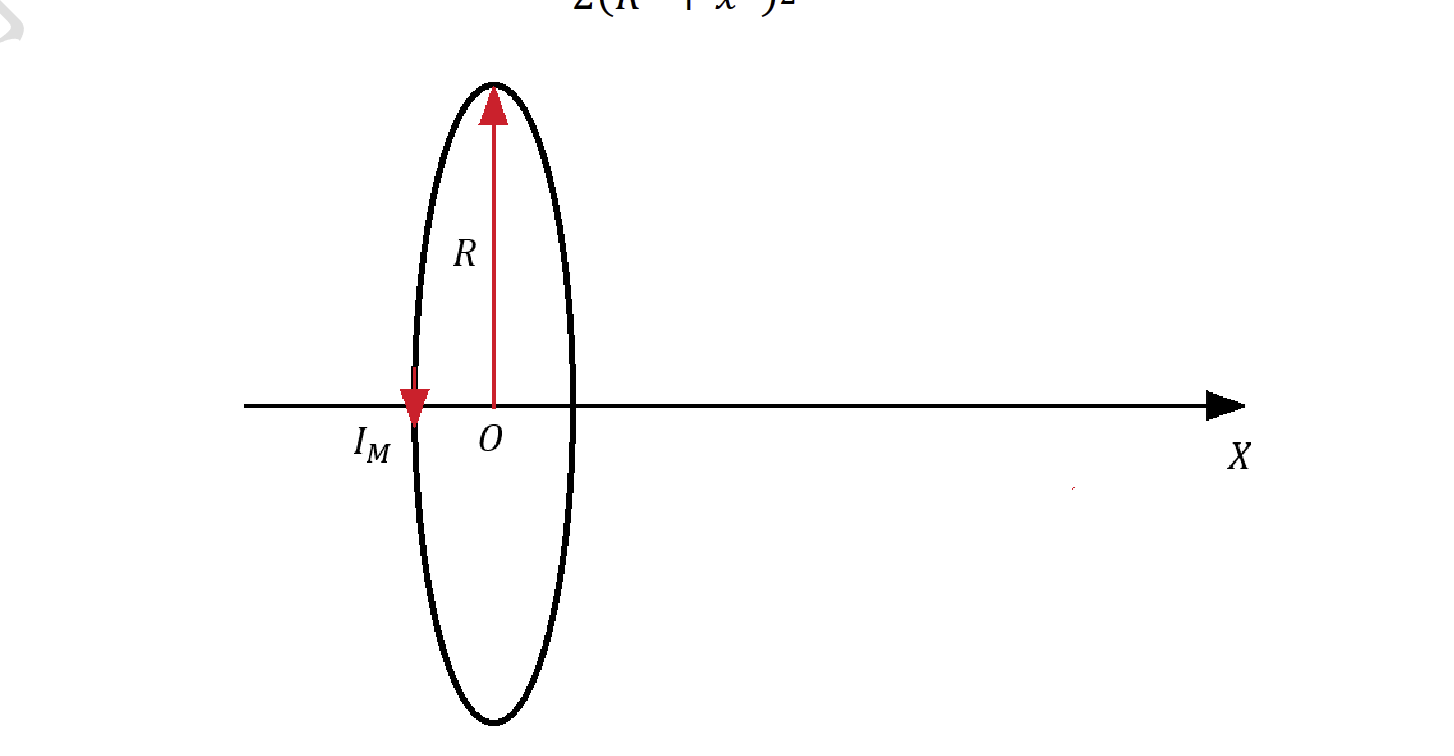
\includegraphics[width=0.7\textwidth]{helmholtz_coil.png}
    \caption{亥姆霍兹线圈示意图}
    \label{fig:helmholtz_coil}
    \end{figure}
    
    对于单个环形线圈,轴线上 $x$ 处的磁感应强度为:
    
    \begin{equation}
    B_x(x) = \frac{\mu_0 N I_M R^2}{2(R^2+x^2)^{3/2}}
    \end{equation}
    
    由磁场叠加原理,双线圈轴线上磁感应强度为:
    
    \begin{equation}
    B_x(x) = \frac{\mu_0 N I_M R^2}{2} \left[ \frac{1}{(R^2+(x+d/2)^2)^{3/2}} + \frac{1}{(R^2+(x-d/2)^2)^{3/2}} \right]
    \end{equation}
    
    可以证明,当两线圈间距等于线圈半径时,中心处 $x=0$ 满足 $\frac{\partial B_x}{\partial x}=\frac{\partial^2 B_x}{\partial x^2}=\frac{\partial^3 B_x}{\partial x^3}=0$,磁场最为均匀。
    
    \subsection{铁球在均匀磁场中的感应磁场}
    
    将一个半径为 $R$ 的铁球置于感应强度为 $\vec{B}_0=(B_0,0,0)$ 的均匀磁场中,铁球会产生感应磁化,其磁化强度 $\vec{M}$ 与外加磁场 $\vec{B}_0$ 同方向。设真空磁导率为 $\mu_0$,铁球的相对磁导率为 $\mu_r$,铁球内部感应磁场 $\vec{B}$ 满足:
    
    \begin{equation}
    \vec{B} = \mu_0(\vec{H}_0+\vec{M}) = \mu_0\left(\frac{\vec{B}_0}{\mu_0}+\frac{\mu_r-1}{\mu_r+2}\vec{B}_0\right) = \frac{3\mu_r}{\mu_r+2}\vec{B}_0 \approx 3\vec{B}_0 \quad (\mu_r \gg 1)
    \end{equation}
    
    即铁球内部磁场是外加磁场的3倍。
    
    在铁球外部,感应磁场 $\vec{B}_e$ 相当于一个磁偶极子的磁场。取铁球中心为坐标原点,z轴与外加磁场同向,则铁球表面磁荷密度 $\sigma_m=\frac{3\mu_0}{4\pi}\vec{M}\cdot\vec{e}_r=\frac{3B_0}{4\pi}\cos\theta$,其中 $\theta$ 为 $\vec{e}_r$ 与 $z$ 轴的夹角。由磁偶极子的磁位计算公式,真空中一点 $P(r,\theta)$ 处感应磁场为:
    
    \begin{equation}
        \vec{B}_e(P) = 
        \begin{cases}
            (2B_0,0,0) & r \leq R \\
            \frac{\mu_0}{4\pi}\frac{1}{r^3} \left[ \frac{3R^3B_0}{r^3}(2\cos^2\theta-\sin^2\theta)\vec{e}_r + \frac{3R^3B_0}{r^3}\sin\theta\cos\theta\vec{e}_{\theta} \right] & r > R
        \end{cases}  
    \end{equation}
    
    沿轴线 ($\theta=0$ 或 $\pi$) 方向,感应磁场与外加磁场同向,磁场加强;在赤道面 ($\theta=\pi/2$) 上,感应磁场与外加磁场反向,磁场减弱。总磁场是外加磁场与感应磁场的矢量和。


    \section{实验过程}

    \subsection{霍尔效应验证及灵敏度测量}
    
    \subsubsection{实验装置搭建}
    将两个线圈按照亥姆霍兹线圈的要求组装,并将霍尔传感器放置在线圈中心。调节电源输出,左路恒流源为线圈提供励磁电流 $I_M$,右路恒流源为霍尔元件提供工作电流 $I_S$。读取显示数据见识两路电流。
    
    \subsubsection{霍尔电压与磁场关系测量} \label{sec:hall_effect_Im}
    固定 $I_S=10mA;\ d=R$,改变 $I_{Mtotal}$ 从 $0\sim1000mA$,每隔 $20mA$ 记录对应的 $B$ 和 $V_H$。由于
    \begin{equation}
        B_{center}(I_M) = \frac{\mu_0 N I_M R^2}{(R^2+(R/2)^2)^{3/2}} 
    \end{equation}
    $I_M$ 和 $B$ 成正比,改变 $I_M$ 即可得到不同的 $B_{center}$ 值。
    其中,由于励磁电流供给两路线圈,故实际励磁电流 $I_{Mtotal}=2I_M$。

    在每个 $I_M$ 下,需要测量 4 种 $I_S$ 和 $I_M$ 组合下的霍尔电压,然后按照
    \begin{equation}
    V_H = \frac{1}{4}(U_{++} - U_{+-} + U_{--} - U_{-+})
    \end{equation} 
    计算 $V_H$,消除其他效应的影响。
    测量记录数据如下:

    \begin{table}[htbp]
        \centering
        \caption{霍尔电压与磁场关系测量数据记录}
        \begin{tabular}{l|llllll}
            No.&I\_m(mA)&U++(mV)&U--(mV)&U+-(mV)&U-+(mV)&V\_h(mV)\\
            \hline
            1&10&-1.28&2.35&2.21&-1.41&0.07\\
            2&20&-1.21&2.41&2.14&-1.48&0.13\\
            3&30&-1.14&2.48&2.08&-1.54&0.20\\
            4&40&-1.08&2.54&2.01&-1.63&0.27\\
            5&50&-1.01&2.61&1.94&-1.69&0.34\\
            6&60&-0.94&2.68&1.89&-1.76&0.40\\
            7&70&-0.88&2.75&1.82&-1.83&0.47\\
            8&80&-0.81&2.81&1.75&-1.89&0.53\\
            9&90&-0.74&2.88&1.69&-1.95&0.60\\
            10&100&-0.68&2.95&1.63&-2.03&0.67\\
            11&110&-0.61&3.03&1.55&-2.08&0.74\\
            12&120&-0.55&3.08&1.48&-2.14&0.80\\
            13&130&-0.48&3.16&1.43&-2.21&0.87\\
            14&140&-0.42&3.22&1.35&-2.28&0.93\\
            15&150&-0.34&3.29&1.28&-2.36&1.01\\
            16&160&-0.28&3.36&1.22&-2.41&1.07\\
            17&170&-0.21&3.43&1.15&-2.48&1.14\\
            18&180&-0.14&3.49&1.09&-2.56&1.21\\
            19&190&-0.08&3.56&1.02&-2.62&1.27\\
            20&200&-0.01&3.63&0.95&-2.68&1.34\\
            21&210&0.06&3.69&0.89&-2.73&1.40\\
            22&220&0.13&3.76&0.81&-2.81&1.47\\
            23&230&0.19&3.83&0.74&-2.88&1.54\\
            24&240&0.27&3.89&0.68&-2.95&1.61\\
            25&250&0.33&3.96&0.61&-3.01&1.67\\
            26&260&0.39&4.03&0.54&-3.08&1.74\\
            27&270&0.46&4.10&0.49&-3.14&1.80\\
            28&280&0.53&4.16&0.42&-3.21&1.87\\
            29&290&0.59&4.23&0.36&-3.27&1.93\\
            30&300&0.66&4.29&0.30&-3.34&2.00\\
            31&310&0.73&4.36&0.22&-3.41&2.07\\
            32&320&0.79&4.43&0.16&-3.48&2.14\\
            33&330&0.87&4.49&0.09&-3.54&2.20\\
            34&340&0.93&4.56&0.03&-3.60&2.26\\
            35&350&0.99&4.62&-0.06&-3.68&2.34\\
            36&360&1.06&4.69&-0.11&-3.74&2.40\\
            37&370&1.12&4.74&-0.17&-3.81&2.46\\
            38&380&1.20&4.83&-0.24&-3.88&2.54\\
            39&390&1.26&4.89&-0.30&-3.94&2.60\\
            40&400&1.33&4.95&-0.36&-4.01&2.66\\
            \end{tabular}
    \end{table}
    \newpage
    \begin{figure}[htbp]
        \centering
        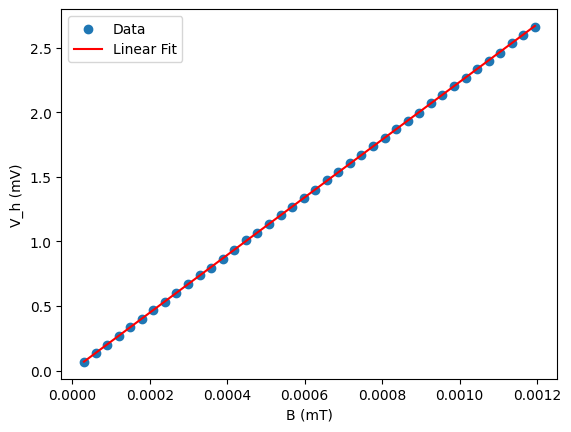
\includegraphics[width=0.7\textwidth]{hall_effect_Im.png}
        \caption{测量霍尔电压与磁场关系图}
        \label{fig:hall_effect_Im}
    \end{figure}
    数据记录完毕后,以 $B$ 为横轴,$V_H$ 为纵轴作图,如图\ref{fig:hall_effect_Im}。根据理论分析,两者应呈线性关系:
    \begin{equation}
    V_H = K_H I_S B_{center}
    \end{equation}
    用最小二乘法拟合直线$V_h = A_m \cdot B + b_m$,斜率即为灵敏度与霍尔电流的乘积 $K_H \cdot I_s$。
    回归得到,数值:
    \begin{equation}
        K_H \cdot I_s = \SI{2230.91}{V/T}
    \end{equation}
    
    \subsubsection{霍尔电压与工作电流关系测量}
    固定 $I_M=1000mA$,改变 $I_S$ 从 $0\sim10mA$,每隔 $0.5mA$ 记录对应的 $I_S$ 和 $V_H$。测量步骤与数据处理方法同上。
    
    作 $V_H-I_S$ 图,两者应呈线性关系,斜率为 $K_H B$。结合已知的 $K_H I$ 值,可计算 $K_H$。
    
    \begin{figure}[htbp]
        \centering
        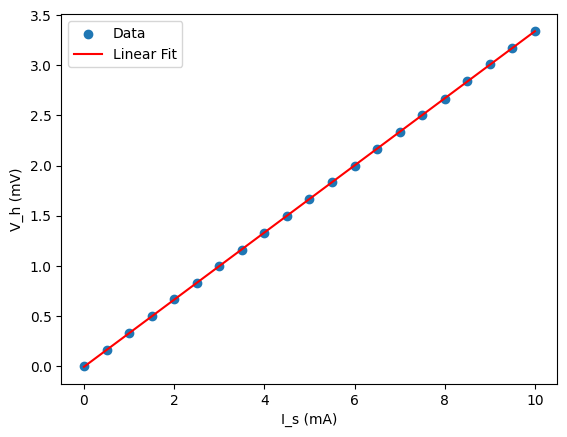
\includegraphics[width=0.5\textwidth]{hall_effect_Is.png}
        \caption{测量霍尔电压与霍尔电流关系图}
        \label{fig:hall_effect_Is}
    \end{figure}
    
    记录原始数据如下:
    \begin{table}[htbp]
        \centering    
        \begin{tabular}{l|llllll}
        No.&I\_s(mA)&U++(mV)&U--(mV)&U+-(mV)&U-+(mV)&$V_h$(mV)\\
        \hline
        1&0&-0.31&-0.31&-0.31&-0.31&0\\
        2&0.50&-0.20&-0.03&-0.36&-0.52&0.16\\
        3&1&-0.08&0.27&-0.39&-0.74&0.33\\
        4&1.50&0.03&0.56&-0.44&-0.96&0.50\\
        5&2&0.15&0.85&-0.48&-1.18&0.67\\
        6&2.50&0.26&1.14&-0.52&-1.39&0.83\\
        7&3&0.38&1.43&-0.56&-1.62&1.00\\
        8&3.50&0.49&1.72&-0.60&-1.84&1.16\\
        9&4&0.61&2.01&-0.64&-2.05&1.33\\
        0&4.50&0.72&2.31&-0.69&-2.25&1.49\\
        11&5&0.84&2.59&-0.73&-2.49&1.66\\
        12&5.50&0.95&2.89&-0.78&-2.71&1.83\\
        13&6&1.06&3.18&-0.82&-2.93&2.00\\
        14&6.50&1.18&3.48&-0.86&-3.13&2.16\\
        15&7&1.29&3.78&-0.90&-3.38&2.34\\
        16&7.50&1.41&4.06&-0.94&-3.60&2.50\\
        17&8&1.53&4.36&-0.98&-3.80&2.67\\
        18&8.50&1.65&4.66&-1.01&-4.04&2.84\\
        19&9&1.76&5.01&-1.04&-4.26&3.02\\
        20&9.50&1.87&5.26&-1.08&-4.48&3.17\\
        21&10&1.99&5.58&-1.11&-4.70&3.34\\
        \end{tabular}
    \end{table}    
    数据记录完毕后,以 $I_s$ 为横轴,$V_H$ 为纵轴作图,如图\ref{fig:hall_effect_Is}。根据理论分析,两者应呈线性关系:
    \begin{equation}
    V_H = K_H I_S B_{center}
    \end{equation}
    用最小二乘法拟合直线$V_h = A_s \cdot I_s + b_s$,斜率即为灵敏度与霍尔电流的乘积 $K_H \cdot B_{center}$。
    回归得到,数值:
    \begin{equation}
        K_H \cdot B_{center} = \SI{0.3347}{V/A}
    \end{equation}
    进一步计算得到:
    \begin{equation}
        K_H = \sqrt{\frac{A_m \cdot A_s}{I_s \cdot B_{center}}} = \SI{86.41}{VT^{-1}A^{-1}}
    \end{equation}
    \subsection{亥姆霍兹线圈磁场分布测量}
    \subsubsection{建立 $V_H-U_{++}$ 关系}
    根据上一节\ref{sec:hall_effect_Im}的测量结果,建立 $V_H$ 与 $U_{++}$ 的对应关系。
    首先,绘制$V_H-U++$的相关图像,并进行拟合。相关性如图\ref{fig:VH-U++}:
    \begin{figure}[htbp]
        \centering
        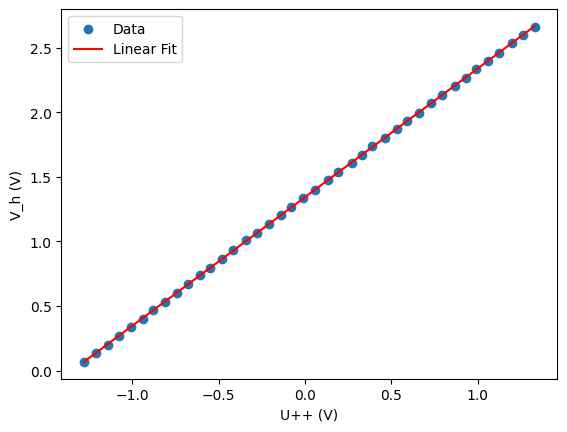
\includegraphics[width=0.5\textwidth]{VH-U++.png}
        \caption{VH-U++关系图}
        \label{fig:VH-U++}
    \end{figure}
    可采用线性拟合:
    \begin{equation}
    V_H = k U_{++} + b    
    \end{equation}
    拟合得到:
    \begin{equation}
        \label{eq:0}
        V_H = 0.996 \cdot U_{++} + \SI{1.344}{V}
    \end{equation}
    线性模型拟合优度即较高,后续只需测量 $U_{++}$ 即可代入\ref{eq:0}间接得到 $V_H$。
    
    \subsubsection{磁场分布测量} \label{sec:measure}
    固定 $I_M=1000mA$,将两励磁线圈间隔为R摆放,沿线圈轴线方向移动霍尔传感器,每隔 $\SI{5}{mm}$ 测量 $U_{++}$,并换算为 $B$。以轴线坐标 $x$ 为横轴,$B$ 为纵轴作图,得到磁场分布曲线。
    
    \begin{figure}[htbp]
    \centering
    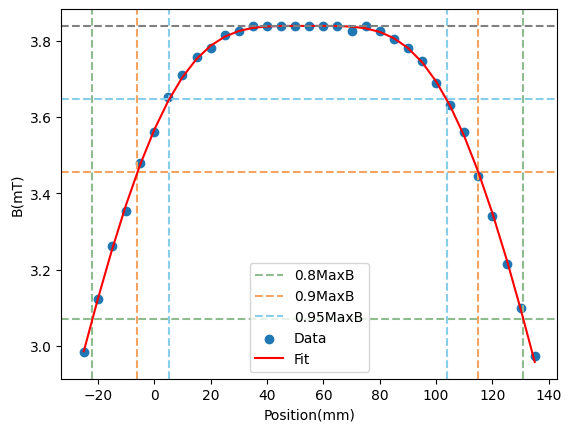
\includegraphics[width=0.6\textwidth]{B-x.png}
    \caption{亥姆霍兹线圈轴线上磁场分布}
    \label{fig:B-x}
    \end{figure}
\newpage
    从曲线上找出磁场最大值 $B_{max}$,分别计算 $0.95B_{max}$、$0.9B_{max}$ 和 $0.8B_{max}$ 对应的 $x$ 坐标分别为:
    \begin{table}[htbp]
        \centering
        \begin{tabular}{|l|l|l|l|}
            \hline
            均匀度&0.95&0.9&0.8\\
            \hline
            范围(mm)&98.46&121.08&152.94\\
            \hline
        \end{tabular}
    \end{table}
    \\
    \subsection{铁球感应磁场测量}
    将铁球置于亥姆霍兹线圈中心,调节 $I_M=1000mA$,测量轴线上不同位置的磁感应强度 $B_{total}$。由于
    \begin{equation}
    \vec{B}_{total} = \vec{B}_0 + \vec{B}_e     
    \end{equation}
    为了得到铁球的感应磁场 $\vec{B}_e$,需要扣除外加磁场 $\vec{B}_0$。
    使用测量结果扣除\ref{sec:measure}中测量得到的背景场数据,且推测中心点得到导出的x,并使用函数$B = \frac{A}{(x-B)^3}+C$进行拟合
    
    得到如下结果:
    \begin{figure}[htbp]
        \centering
        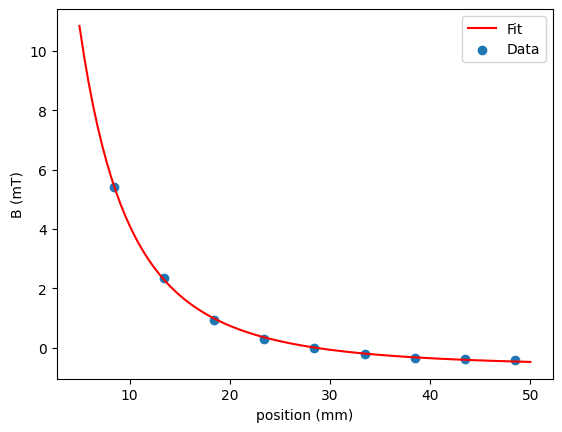
\includegraphics[width=0.4\textwidth]{B-xball.png}
        \caption{铁球感应磁场分布}
        \label{fig:B-x}
    \end{figure}
\\
    \begin{table}[htbp]
        \centering
        \begin{tabular}{|l|l|l|l|}
            \hline
            参数&A&B&C\\
            \hline
            数值&36314.5&-9.92&0.07\\
            \hline
        \end{tabular}
    \end{table}
    \\
    将测量结果与理论计算公式对比:
    \begin{equation}
    \vec{B}_e(x) = \frac{2R^3 B_0}{x^3}\vec{e}_x \quad (x > R)
    \end{equation}
    其中 $R$ 为铁球半径,$x$ 为距离铁球中心的距离,A的理论值应为:39437,与实验值相差约为:$8.6\%$。
    
    \section{误差分析}
    \begin{enumerate}
        \item 由于实验环境的影响,霍尔元件的输出电压可能受到其他效应的影响,导致实验结果与理论值有一定偏差。
        \item 由于铁球的非理想性,磁导率不可能为无穷大,实验测量的结果与理论值有一定偏差。
        \item 由于实验仪器的精度限制,实验结果与理论值有一定偏差。
        \item 由于实验中大量参数为实际测得,并且误差传递较为复杂且积累较大,可能导致最中测量结果不理想
    \end{enumerate}
    
\end{document}



